\chapter{Bakground}



\section{Reinforcement Learning and Markov Decision Processes}

Sequential Decision Probles have often ha

Reinforcement Learning is a learning paradigm, though often is also defined as a learning problem itself \citep{Todorov2006}, that commonly assumes an underlying Markov Decision Process (MDP). An MDP is a tuple ${\cM = \langle\cS,\cA,\cR,\mathbb{P},\mathbb{P}_0\rangle}$. Here
\begin{itemize}
    \item $\cS$ is the set of states.
    \item $\cA$ is the set of actions.
    \item $\cR:\cS\times\cA\times\cS\rightarrow\real$ is a reward function. In this defintion, the reward function maps transitions $(s, a, s')\in\cS\times\cA\times\cS$ to scalars, however this 
    \item $\mathbb{P}:\cS\times\cA\rightarrow\Delta(\cA)$ is the transition probabality function.
    \item $\mathbb{P_0}:\Delta(S)$ is the initial state distribution.
\end{itemize}
The RL learning loop is typically illustrated with Figure~\ref{fig:rl_loop}. It shows an agent that interacts with an environment in a sequential fashion: it observes a state $S_t$, selects action $A_t$ according to policy $\pi_t$ and the environment returns a scalar reward $\cR_{t+1}$ and a new state $S_{t+1}$.


\begin{figure}
    \centering
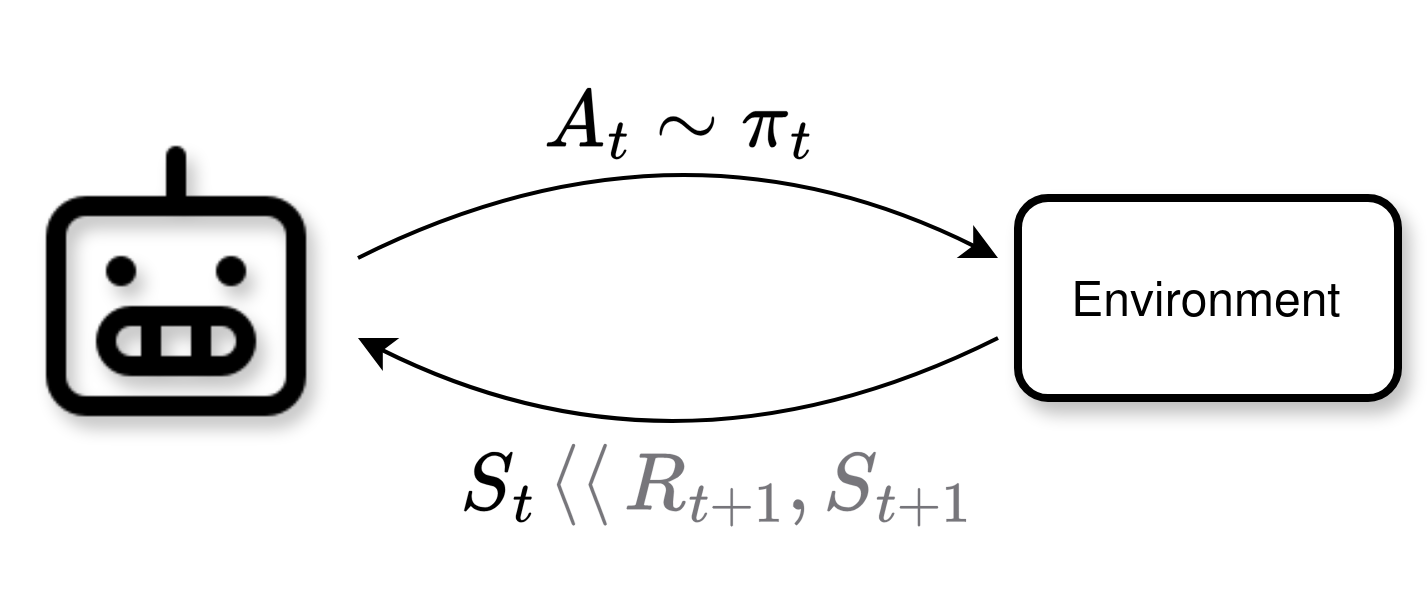
\includegraphics[width=0.65\textwidth]{figures/RL_loop.png}
    \caption{Caption}
    \label{fig:rl_loop}
\end{figure}

\section{Linearly-solvable Reinforcement Learning}


\section{Background}

%In this section we present the necessary background for our work and introduce notation used throughout.

Given a finite set $\cX$, let $\Delta(\cX)=\{p\in\real^\cX:\sum_x p(x)=1,\linebreak p(x)\geq 0\;(\forall x)\}$ denote the probability simplex on $\cX$. Given a probability distribution $p\in\Delta(\cX)$, let $\cB(p)=\{x\in\cX:p(x) > 0\}\subseteq\cX$ denote the support of $p$.


\subsection{Linearly-Solvable Markov Decision Processes}

A linearly-solvable Markov decision process, or LMDP~\citep{Todorov2006}, can be defined as a tuple $\cL=\langle\cS,\cT,\cP,\cR,\cJ\rangle$, where $\cS$ is a set of non-terminal states, $\cT$ is a set of terminal states, $\cP:\cS\rightarrow\Delta(\cS^+)$ is an uncontrolled transition function, $\cR:\cS\rightarrow\real$ is a reward function for non-terminal states, and $\cJ:\cT\rightarrow\real$ is a reward function for terminal states. We use $\cS^+=\cS\cup\cT$ to denote the full set of states, and $S^+=|\cS^+|$ (resp.~$S=|\cS|$) to denote the number of (non-terminal) states. 
We also use $B=\max_{s\in\cS}|\cB(\cP(\cdot|s))|$ to denote an upper bound on the support of $P$.

The learning agent follows a policy $\pi:\cS\rightarrow\Delta(\cS^+)$ that, for each non-terminal state $s\in\cS$, chooses a probability distribution over next states in the support of $\cP(\cdot|s)$, i.e.~$\pi(\cdot|s)\in\Delta(\cB(\cP(\cdot|s))$. In each round $t$, the learning agent observes a state $s_t\in\cS^+$. If $s_t$ is non-terminal, the agent transitions to a new state $s_{t+1}\sim\pi(\cdot|s_t)$ and receives an immediate reward
\[
\cR(s_t,\pi) = \cR(s_t) - \lambda\cdot\mathrm{KL}(\pi(\cdot|s_t)\Vert\, \cP(\cdot|s_t)),
\]
where $\cR(s_t)$ is the reward associated with state $s_t$, $\mathrm{KL}(\pi(\cdot|s_t)\Vert\, \cP(\cdot|s_t))$ is the Kullback-Leibler divergence between $\pi(\cdot|s_t)$ and $\cP(\cdot|s_t)$, and $\lambda$ is a temperature parameter. Hence the agent can set the probability distribution $\pi(\cdot|s_t)$ freely, but gets penalized for deviating from the uncontrolled distribution $\cP(\cdot|s_t)$. On the other hand, if $s_t$ is terminal, the agent receives reward $\cJ(s_t)$ and then the current episode ends. The aim of the agent is to compute a policy $\pi$ that maximizes the expected future reward (i.e.~value), defined in each non-terminal state $s\in\cS$ as
\[
v^\pi(s) = \EEc{\sum_{t=1}^{T-1} \cR(S_t,\pi) + \cJ(S_T)}{S_1 = s}.
\]
Here, $T$ is a random variable representing the time at which the current episode ends, and $S_t$ is a random variable representing the state at time $t$. The expectation is over the stochastic choice of next state $S_{t+1}\sim\pi(\cdot|S_t)$ at each time~$t$, and the time $T$ it takes for the episode to end. We assume that the reward of all non-terminal states is negative, i.e.~$\cR(s)<0$ for each $s\in\cS$. As a consequence, $\cR(s,\pi)<0$ holds for any policy $\pi$, and the value $v^\pi(s)$ has a well-defined upper bound. %As an alternative to the assumption $\cR(s)<0$, we could instead assume that each policy terminates with probability 1 within a fixed time horizon $H$.

We are interested in computing the optimal value function $v^*:\cS\rightarrow\real$, i.e.~the maximum expected future reward among all policies. For simplicity, in what follows we omit the asterisks and refer to the optimal value function simply as the value function. We extend the value function to each terminal state $\tS\in\cT$ by defining $v(\tS)\equiv\cJ(t)$. The value function $v$ satisfies the Bellman equations
\begin{align*}
& \frac 1 \lambda v(s) = \frac 1 \lambda \max_\pi \left[ \cR(s,\pi) + \mathbb{E}_{s'\sim\pi(\cdot|s)} v(s') \right] \\
 &= \frac{1}{\lambda} \cR(s) + \max_\pi \mathbb{E}_{s'\sim\pi(\cdot|s)} \left[ \frac 1 \lambda v(s') - \log \frac {\pi(s'|s)} {\cP(s'|s)} \right] \;\; \forall s.
\end{align*}
We introduce the notation $z(s)=e^{v(s)/\lambda}$ for each $s\in\cS^+$, and often abuse notation by referring to $z(s)$ as the (optimal) value of $s$. The maximization in the Bellman equations can be resolved analytically, yielding the following Bellman equations that are linear in $z$:
\begin{equation}\label{eq:z}
z(s) = e^{\cR(s)/\lambda} \sum_{s'}\cP(s'|s)z(s').
\end{equation}
We can express the Bellman equation in matrix form by defining an $S\times S$ diagonal reward matrix $R=\diag(e^{\cR(\cdot)/\lambda})$ and an $S\times S^+$ stochastic transition matrix $P$ whose entries $(s,s')$ equal $\cP(s'|s)$. We also define a vector $\bf z$ that stores the values $z(s)$ for each non-terminal state $s\in\cS$, and a vector $\bf z^+$ extended to all states in $\cS^+$. We can now write the Bellman equations in matrix form:
\begin{equation}\label{eq:matrixz}
{\bf z} = R P {\bf z^+}.
\end{equation}
Given $z$, the optimal policy $\pi$ is given by the following expression for each pair of states $(s,s')$:
\begin{equation}\label{eq:pi}
\pi(s'|s) = \frac {\cP(s'|s)z(s')} {\sum_{s''} \cP(s''|s)z(s'')}.
\end{equation}

The solution for $z$ corresponds to the largest eigenvector of $RP$.
If the dynamics $\cP$ and $\cR$ are known, we can iterate~\eqref{eq:matrixz}~\citep{Todorov2006}.
Alternatively, we can incrementally learn an estimate $\hat{z}$ using stochastic updates based on state transitions sampled from the uncontrolled dynamics $(s_t,r_t,s_{t+1})$
% use an online algorithm called Z-learning to compute an estimate  \citep{TodorovNIPS2007}. After observing each transition , the update rule of Z-learning is given by
\[
\hat{z}(s_t) \leftarrow (1-\alpha_t)\hat{z}(s_t) + \alpha_t e^{r_t/\lambda}\hat{z}(s_{t+1}),
\]
where $\alpha_t$ is a learning rate. 
The above update rule is called Z-learning~\citep{Todorov2006} and suffers from slow convergence in very large state spaces and when the optimal policy differs substantially from the uncontrolled dynamics $\cP$.
%assumes that we sample next states using the uncontrolled transition function $\cP$, which is typically no better than a random walk. 
A better choice is importance sampling, which uses samples from the estimated policy $\hat{\pi}$ derived from the estimated values $\hat{z}$ and \eqref{eq:pi} and updates $\hat{z}$ according to the following update
%to obtain samples that are corrected using the following update~\citet{TodorovPNAS2009}:
%to sample In this case,  suggested a corrected update rule based on importance sampling:
\begin{align}\label{eqn:zlearning-imp}
\hat{z}(s_t) \leftarrow (1-\alpha_t)& \hat{z}(s_t) + \alpha_t e^{r_t/\lambda}\hat{z}(s_{t+1})\frac {\cP(s_{t+1}|s_t)} {\hat{\pi}(s_{t+1}|s_t)}.
\end{align}
However, this requires local knowledge of $\cP(\cdot|s_t)$ to correct for the different sampling distribution.
%, i.e.~the set of possible next states and their associated uncontrolled probabilities.
Though this seems like a strong assumption, in practice $\cP$ usually has a simple form, e.g.~a random walk.
Further, as shown in \citet{Jonsson2016}, the corrected update rule in \eqref{eqn:zlearning-imp} can also be used to perform off-policy updates in case transitions are sampled using a policy different from $\hat{\pi}$,
%leading to simultaneous learning of different tasks.
%Note that the expression for the policy $\hat{\pi}$ in \eqref{eq:pi} and the corrected update rule in \eqref{eqn:zlearning-imp} require local knowledge of $\cP(\cdot|s_t)$, i.e.~the set of possible next states and their associated uncontrolled probabilities. Though this seems like a strong assumption, in practice $\cP$ usually has a simple form, e.g.~uniform. \citet{conf/icaps/Jonsson16} showed that the corrected update rule in \eqref{eqn:zlearning-imp} can also be used to perform off-policy updates in case transitions are sampled using a policy different from $\hat{\pi}$.

\subsection{Compositionality}

\citet{Todorov2009a} introduced the concept of compositionality for LMDPs. Consider a set of LMDPs $\{\cL_1,\ldots,\cL_n\}$, where each LMDP $\cL_i=\langle\cS,\cT,\cP,\cR,\cJ_i\rangle$ has the same components $\cS,\cT,\cP,\cR$ and only differ in the reward $\cJ_i(\tS)$ of each terminal state $\tS\in\cT$, as well as its exponentiated value $z_i(\tS)=e^{\cJ_i(\tS)/\lambda}$.

Now consider a new LMDP $\cL=\langle\cS,\cT,\cP,\cR,\cJ\rangle$ with the same components as the $n$ LMDPs above, except for $\cJ$. Assume that there exist weights $w_1,\ldots,w_n$ such that the exponentiated value of each terminal state $\tS\in\cT$ can be written as
\[
e^{\cJ(\tS)/\lambda} = z(\tS) = w_1z_1(\tS) + \ldots + w_nz_n(\tS) = \sum_{k=1}^n w_kz_k(\tS).
\]
Since the Bellman optimality equation of each non-terminal state $s\in\cS$ is linear in $z$, the optimal value of $s$ satisfies the same equation:
\[
z(s) = \sum_{k=1}^n w_kz_k(s).
\]
Consequently, if we previously compute the optimal values $z_1,\ldots,z_n$ of the $n$ LMDPs and know the weights $w_1,\ldots,w_n$, we immediately obtain the optimal values of the new LMDP $\cL$ without learning.




\section{Hierarchical Reinforcement Learning}
\subsection{Optimality of HRL algorithms}
\cite{Dietterich2000} identifies two types of optimality for hierarchical methods in reinforcement learning, namely \textit{hierarchical optimality} and \textit{recursive optimality}. Hierarchical optimality implies optimality with regard a constrained space of policies, given by the hierarchy structure. Hierarchies of Abtract Machines (HAMs,~\cite{Parr1997}) and the Options Framework~\citep{Sutton1999} lie in this category) 


\section{Non-Markovian Reinforcement Learning and Task Specification}

